\pdfoutput=1
\RequirePackage{amsmath}
\documentclass[iop, apj]{emulateapj}
\usepackage[varg]{newtxmath}
\usepackage{newtxtext}
\usepackage[spanish,es-minimal,english]{babel}
\usepackage[utf8]{inputenc}
\usepackage{natbib}
\usepackage{microtype}
\usepackage{hyperref}
\graphicspath{ {figs/}, {../}, {../luis-programas}}
\bibliographystyle{apj}

\begin{document}
\title{
  The interlocking spiral structure of the Orion Nebula
}
\author{
  William J. Henney, 
  Luis A. Gutiérrez-Soto,
  Jorge A. Tarango-Yong 
}
\affil{%
  \foreignlanguage{spanish}{Centro de Radioastronomía y
    Astrofísica, Universidad Nacional Autónoma de México, Apartado
    Postal 3-72, 58090 Morelia, Michaoacán, Mexico};
  w.henney@crya.unam.mx, l.gutierrez@crya.unam.mx,
  j.tarango@crya.unam.mx}


\begin{abstract}
  We show that the 
  Drawing on recent studies of stellar bowshocks in the Orion Nebula,
  we show that the flow of gas in the nebula has 
\end{abstract}

\begin{figure}
  \centering
  \includegraphics[width=\linewidth]{spiral-bars}
  \caption{The interlocking spirals.}
  \label{fig:spiral-bars}
\end{figure}

\begin{figure*}
  \centering
  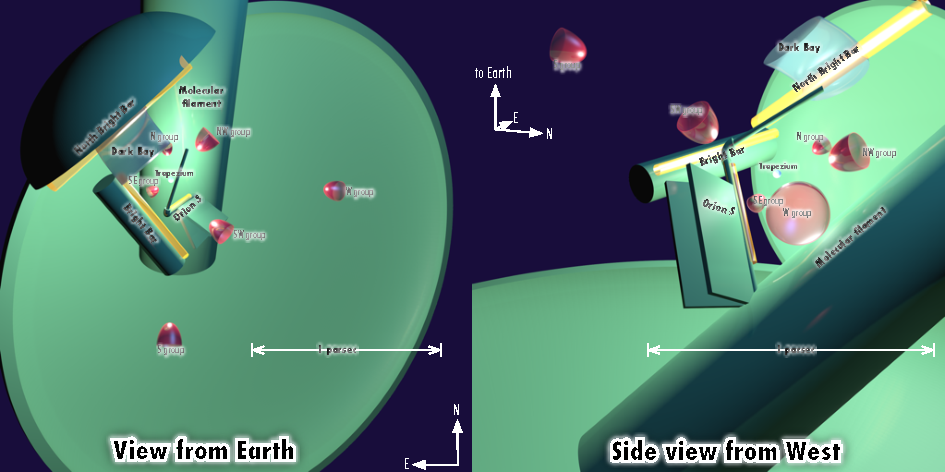
\includegraphics[width=\linewidth]{orion-3d-twin-view}
  \caption{Simplified three-dimensional structure of the Orion Nebula.}
  \label{fig:3d-twin}
\end{figure*}

For clarity, we have omitted many secondary features and slightly increased the
size of the smaller features, such as Orion~South. 
The sizes of the smaller features  of the different features have been modified slighty


\bibliography{BibdeskLibrary-slavoj}


\end{document}

